\chapter{The Kazan School: De Courtenay}
\label{ch.kazan}

A number of years before {\Saussure} began to occupy himself seriously
with questions of general linguistics, many of those very problems
constituted the central concern of the Polish linguist Jan {\DeCourtenay} and his students and colleagues (most notably, \name{Mikołaj}{Kruszewski}).\footnote{A more detailed history of the Kazan' linguists
  and their major works, with extensive references not included here,
  is provided by \citet{radwanska-williams21:kazan}.}  Isolated in
Kazan' in central Russia, {\Baudouin}'s scholarship was largely
inaccessible to scholars in Europe, though it was known to at least a
few of them, including {\Saussure}, whom he met at an 1881 meeting of the
Société linguistique de Paris where he presented some of his and
{\Kruszewski}'s work. In the writings of the so-called Kazan school we
find many of the same positions that would later be attributed to
{\Saussure}, and in many cases {\Baudouin}'s formulation of these issues,
and his discussion and resolution of them, is considerably more
explicit and lucid.

We do not study {\Baudouin} and {\Kruszewski}'s views simply because they
distinguished language from speech and synchrony from diachrony,
however, or because they recognized the difference between phonetic
properties that distinguish words and those that do not; or even
because they were probably the first to use the word `\isi{phoneme}' in ways
similar to its modern senses (as well as the coiners of the word
`morpheme'). Despite the fact that they addressed these issues well
before {\Saussure} did, their importance does not lie in simple
historical priority.

The views of European and American linguists on such matters derive,
by and large, from the form in which they were presented by {\Saussure}
(or, at least, this was widely claimed to be their source). Given the
overwhelming status of {\Saussure} as the eponymous `{culture} bringer' of
modern linguistics, the fact that others had said much the same thing
earlier would entitle the Kazan school to little more than a footnote
of acknowledgement in works concerned with the subsequent development
of those ideas. This is indeed the case for others who could also be
cited as precursors of `modern' ideas, such as the Swiss linguist \name{Jost}{Winteler} (whose \citeyear{winteler76:kerenz} description of the
Schwyzertütsch dialect of Kerenz included an explicit discussion of
what would later be known as the `\isi{phonemic principle}').

Aside from its status as a historical curiosity, there are at least
two much more important reasons for contemporary linguists to study
the theories of the Kazan school, one intrinsic and one historical. On
the one hand, {\Baudouin} and {\Kruszewski} were much more concerned with
notions corresponding to what we would now call `rules' in sound
structure than with the nature of \isi{representations}. They arrived at the
basic problem of how to understand the \isi{sound structure} of natural
languages through the study of ways in which phonetic distinctions
take on meaning-differentiating function by being `morphologized', and
their central focus was on the nature of the relations between such
morphologically linked (or `alternating') forms. Unlike most of those
who would come after them, they dealt primarily with questions of the
\isi{typology} and evolution of alternations rather than with the nature of
the elements which (from a phonological point of view) compose
individual forms. The substance of their treatment presents insights
(notably into the sources and nature of `phonetic \isi{explanation}' in
phonology) which are arguably more profound than many opinions
underlying discussion of the same issues today.

On the other hand, the theoretical proposals and research emphases of
Baudouin's work contributed to the subsequent evolution of
phonological research, though not in a very direct way. While his
teaching in general linguistics remained little known in western
Europe and America until fairly recently, he did contribute
significantly through his students to the formation of one of the two
major schools of linguistic thought in Russia: the St. Petersburg
(later Leningrad) school. As such, he exerted a subtle and indirect
influence on those linguists studying in Russia who would later form
the {nucleus} of the {Linguistic Circle of Prague}, one of the central
sources for present-day linguistic ideas. Though somewhat tortuous,
there is a path from the proposals of {\DeCourtenay} to the
basic assumptions of {\Trubetzkoy} and {\Jakobson} about the nature of
language; and it is worth studying the former if we wish to understand
the latter.

\section{Biographical remarks}

Although {\Baudouin}'s family came originally from the {French}
aristocracy, they had lived in Poland for several generations when
{\Baudouin} was born in 1845 (in Radzymin, near Warsaw); and he himself
felt a great loyalty to Polish cultural and political ideals
throughout his career even though much of his life was spent outside
Poland. After finishing the gymnasium, he began university studies in
Warsaw, where he received a master of arts degree from the
historical-philological faculty in 1866. Like {\Saussure}, he spent a
number of years studying {Indo-European} in various places (Prague,
Berlin, Jena, \isi{Leipzig}, and St. Petersburg) with prominent scholars of
the day including {\Schleicher}, {\Leskien}, {\Brugmann}, and {\Delbruck}. In
1870, he received a doctorate from \isi{Leipzig} for work on the nature of
\isi{analogy}, as well as a second master's degree (this time from
St. Petersburg, where his Polish degree was not recognized) for a
study of fourteenth-century Old Polish.

His supervisor in St. Petersburg, \name{Ismail}{Sreznevskij}, arranged a
position for him there as docent (roughly, assistant professor) of
comparative grammar beginning in 1870. The most notable result of his
years in St. Petersburg seems to have been the opportunity provided by
the {Russian} Academy in 1872 to do field work on Slovenian dialects in
Austria and northern Italy. When it was published in 1875, his study
of the phonetic systems of some of these dialects earned him a {Russian}
doctorate. His political views and his somewhat contemptuous attitude
toward {\Sreznevskij}, however, resulted in his not being able to stay in
St. Petersburg after his initial appointment, and in 1875 he went to
Kazan (first as assistant professor, and after a year as full
professor).

\begin{wrapfigure}{l}{.4\textwidth}
  \includegraphics[width=.9\textwidth]{figures/Jan_Niecisław_Baudouin_de_Courtenay.jpg}
  \caption{Jan Niecisław Baudouin de Courtenay}
  \label{fig:ch.kazan_baudouin}
\end{wrapfigure}
It is difficult to exaggerate the isolation of this provincial Tatar
city in central Russia, and {\Baudouin} was anything but pleased at
having to work there. Nonetheless, it has sometimes been suggested
that this isolation had a liberating and ultimately beneficial effect
on his scholarship: if work appearing in Kazan was unlikely to be
heard of in the intellectual circles of western Europe, it was
correspondingly free of the pressures exerted by the dominant
influences in those circles. Had {\Baudouin} been entirely dependent on
publication in journals controlled by the Neogrammarian figures of his
day, it is unlikely that he would have produced much of what he did in
general linguistics. Indeed, on those occasions when he or his
students did submit work to such publications, it was received with
considerable hostility (which {\Baudouin} seems to have done his best to
exacerbate with his rather sharp pen and abrasive personality). We may
also note that Kazan had been (fifty years earlier) the place where
\name{Nikolai}{Lobachevsky} had published his work on non-Euclidean
geometry. Whatever its frontierlike lack of amenities and distance
from the main streams of academic life, Kazan does not seem to have
been notably discouraging to creativity.

It was during his years in Kazan that {\Baudouin} was most productive in
general linguistics, whether because of his relative youth or because
of his isolation—or because of the excited and stimulating group of
students and followers he had there. Foremost among these was \name{Mikolaj}{Kruszewski}, whose arrival resulted in the formation of the ``Kazan
Linguistic Circle'' as a forum for the discussion of current
linguistic work and with whom {\Baudouin} quickly developed a very close
working relationship. The historical literature in linguistics has
contained a certain amount of discussion of the details of their
collaboration, especially with regard to their relative priority in
developing particular areas of the `Kazan theory'. {\Baudouin}'s own
discussions of these issues are of little help in resolving them,
since he shifts between extravagant praise of {\Kruszewski}'s rigorous
and scientific development of phonological problems, without which
further progress would have been impossible, and the attitude that
``{\Kruszewski} merely gave another, finer form to what he had learned
from some one else'' \citep[150]{baudouin95:attempt}.

\begin{wrapfigure}{r}{.4\textwidth}
  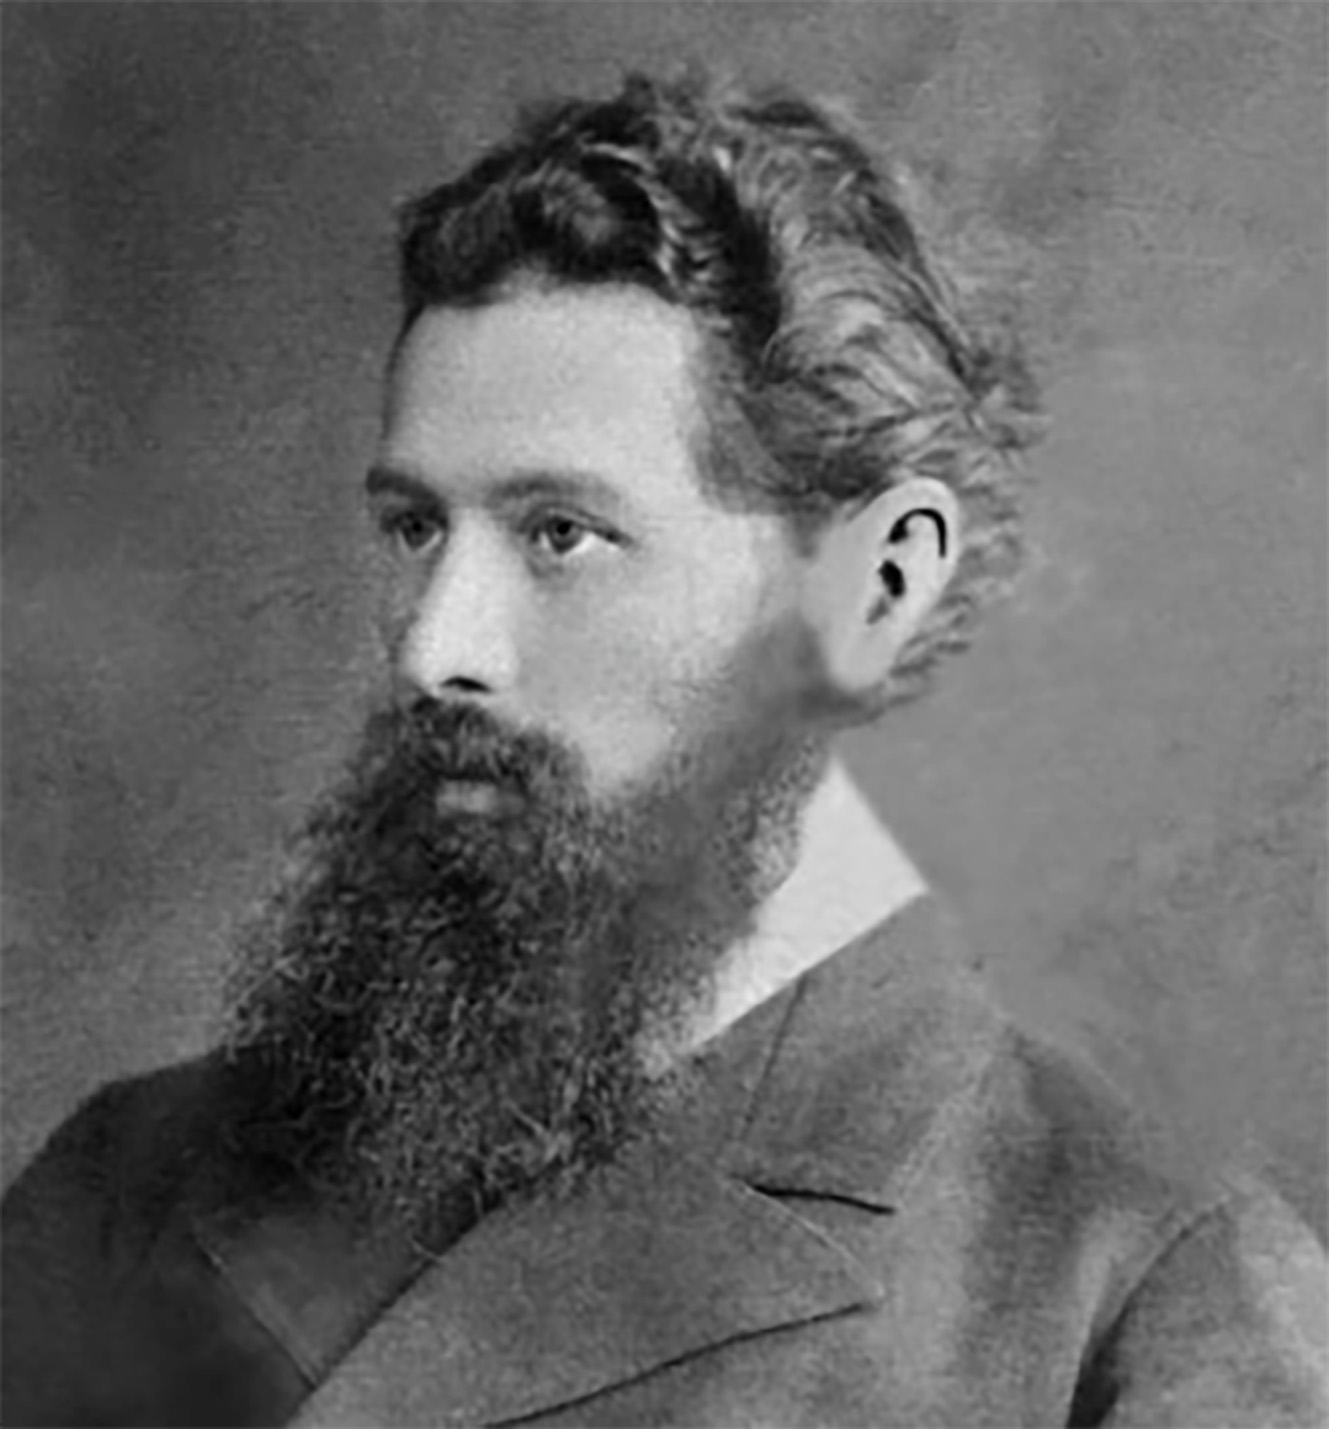
\includegraphics[width=.9\textwidth]{figures/kruszewski.jpg}
  \caption{Mikołaj Kruszewski}
  \label{fig:ch.kazan_kruszewski}
\end{wrapfigure}
Like {\Baudouin}, {\Kruszewski} was born in Poland (in the town of Luck), in
1851. Again like {\Baudouin}, he studied in the historical-philological
faculty in Warsaw, but spent most of his time there reading philosophy
and psychology. He was particularly well trained in {English}
philosophical logic, and the later development of his thought on
linguistic matters would reflect this. After submitting an MA thesis
in 1875 on a folkloristic topic, he wanted to continue his studies in
linguistics, but was financially unable to do so. He had to spend
several years teaching {Russian} language and literature to the
daughters of the provincial nobility before he could take the
suggestion of one of his advisers to go to Kazan in order to study
with {\Baudouin}.

After corresponding with {\Baudouin} for some time and announcing his
interest in developing a genuinely scientific foundation for
linguistics, he arrived in Kazan in 1878 and immediately became an
active participant in {\Baudouin}'s program of research and teaching. He
was awarded a master's degree in 1881 for his thesis on guna
alternations in Old Church Slavonic, a work which contained a
substantial systematic chapter on the theory of alternations (later
published separately in expanded form in {German} as
\citealt{kruszewski81:alternation}) and which {\Baudouin} praised
extravagently in a published review. His 1883 \textsl{Sketch of the
  Science of Language} \citep{kruszewski83:outline}, a rather more
comprehensive if occasionally somewhat tentative work, earned him a
doctorate.

In 1884, {\Kruszewski} fell victim to a progressive degenerative
neurological disorder, probably a complication of syphillis, and spent
the last year and a half of his life in a psychiatric hospital.  It is
evident that {\Baudouin} never managed to come completely to terms with
the premature loss in this way of his young colleague. This is
particularly and painfully clear in the obituary article that {\Baudouin}
wrote about him,\footnote{Now available in translation as
  \citealt{baudouin05:kruszewski-obit-translated}} which can only be
called unbalanced (in more than one sense) and which shows us more
about {\Baudouin}'s state of mind than it does about {\Kruszewski}'s
work. Much of his denigration (here and in later works) of
{\Kruszewski}'s contribution to their joint efforts thus must be seen as
having little necessary connection with the facts.

In any event, there is little point in speculating on the relative
contributions of the two, since it was essentially their joint work
that developed the theoretical position that would subsequently be
presented to others (largely, it is true, through {\Baudouin}'s teaching
and writing). Most of the major themes can already be found in the
programs of {\Baudouin}'s lectures before he had begun to work with
{\Kruszewski}, albeit in very programmatic form. Among these are the
essential difference between the study of speech from a physical
phonetic point of view and the study of the ways in which phonetic
differences serve to distinguish meanings, the importance of the study
of alternations for an understanding of \isi{sound structure}, the relation
between \isi{sound change} and synchronic alternations, etc. It was through
their joint efforts, though, that the substance and interest of the
theory was developed.

In 1883, a chair of comparative Slavic grammar was established in
Dorpat (Tartu, in Estonia), a location which {\Baudouin} found much more
appealing than Kazan and to which he immediately moved. {\Kruszewski}
succeeded {\Baudouin} briefly in the chair of {Indo-European} comparative
grammar in Kazan, but by 1886 his illness had already progressed so
far that he was unable to continue, and he died in the following year.

{\Baudouin}, in turn, became professor of comparative linguistics and
{Sanskrit} in Cracow in 1893, a position which seemed to satisfy his
most intense desires since he was at last in Poland. His pro-Polish
feelings, however, appear to have been somewhat excessive for the
Austro-{Hungarian} authorities, who were hardly supportive of Slavic
nationalism within the empire. Since {\Baudouin} did not enjoy the
equivalent of modern academic tenure, his contract was simply not
renewed after five years, and he was forced to return to
St. Petersburg. Here too he got into political difficulties, this time
through his attacks on the tsarist suppression of national minorities,
and he eventually spent some months in jail. Freed at the outbreak of
World War I, he taught again briefly in St. Petersburg until he was
invited to the chair of {Indo-European} linguistics at the University of
Warsaw in the reestablished postwar independent Poland. He remained
there until his death in 1929.

The influence of {\Baudouin} and {\Kruszewski}, as one might expect, was
primarily on {\Baudouin}'s students, especially in St. Petersburg, where
his teaching was to some extent continued in the Leningrad school of
Soviet linguistics. Their own work, though, was by no means unknown to
linguists outside of their immediate circle. For one thing, unlike
{\Saussure}, {\Baudouin} was intensely interested in detailed problems of
`hands on' \isi{linguistic description} and in the consequences of
theoretical ideas for the solutions to practical problems. He did a
good deal of fieldwork, especially on Slavic dialects, and made a
number of important contributions to comparative Slavic
linguistics. Again unlike {\Saussure}, he published a great deal during
his lifetime; and if, like many others, he never accomplished the
major synthesis of his ideas on general linguistics that he intended,
we are still not at all lacking for direct evidence about his
views. Nonetheless, since much of this body of writing appeared in
rather obscure places and in languages not accessible to many Western
scholars ({Russian} and Polish, in particular), his ideas were not
widely known to his contemporaries.

One exception to this was {\Saussure}, who as mentioned above had met
{\Baudouin} in 1881 at a meeting of the Societe linguistique de
Paris. {\Baudouin} donated copies of some of his and {\Kruszewski}'s works
to the Société and {\Saussure} read them with interest. In his own notes
and manuscripts, {\Saussure} refers on more than one occasion to {\Baudouin}
and {\Kruszewski} as having been ``closer than anyone to a theoretical
view of la \isi{langue}, without departing from purely linguistic
considerations'' \citep[51; my
translation]{godel57:sources}. {\Saussure}'s ideas too, at least in his
earlier work on \ili{Indo-European}, were well known in Kazan. In 1880
{\Kruszewski} had written an enthusiastic review of the \textsl{Mémoire},
and it is apparently from this source that he took the word `\isi{phoneme}'
(then subject to a certain amount of evolution in its sense, which we
will trace below, before it reemerged into the western European
tradition in something like its current acceptation). {\Baudouin}, too,
wrote very favorably about the important innovations of method and
emphasis to be found in the \textsl{Mémoire}.

There was thus a certain amount of interaction, including an exchange
of several letters, as well as mutual appreciation between these two
major sources of modern phonological thought. As far as direct
influence is concerned, however, only {\Saussure}'s work was widely known
until the recent publication of collections of {\Baudouin}'s papers in
Polish \citep{baudouin74f:selected-works} and less fully, in {English}
\citep{baudouin72:stankiewicz-anthology}. A collection of {\Kruszewski}'s
work in {English} translation has been promised for a number of years
but, at this writing, has not yet appeared, although a Polish
collection is available as \citealt{kruszewski67:selected}. Given the
intrinsic interest of much of the Kazan school work, it is unfortunate
that it has been known only through such secondary sources as
\posscitet{jakobson29:remarks,Jakobson60:kazan.school,jakobson65:terms}
review articles; while invaluable, these inevitably reflect Jakobson's
own strongly held views on what is and is not valuable in {\Baudouin}'s
and {\Kruszewski}'s work.

\section{The study of sound systems in the Kazan school}

Just as many of {\Saussure}'s views grew out of his training in
(neogrammarian) historical linguistics, much of what {\Baudouin} and
{\Kruszewski} say about issues in general linguistics reflects their
education and the opinions of the late-nine\-teenth-century linguistic
community of which they were an isolated part. None\-the\-less, even from
his inaugural lecture at St. Petersburg, {\Baudouin} establishes major
differences of emphasis between his approach to the study of language
and that of others. He suggests, in somewhat caricatural form, a
number of different possible goals and methods for such studies, all
of which must be rejected as inadequate or insufficient
(\citet{baudouin71:general-remarks}; quotations below are from the
1972 {English} translation).

The linguist must not be content simply to amass data of a descriptive
sort about particular languages ``without attempting to explain their
causes,'' since this attitude ``avoid[s] the question of the usefulness
and goal of gathering data'' and ``reduces science to a purely empirical
endeavor, to some sort of meaningless game.'' On the other hand, the
tradition of aprioristic, philosophical grammar, ``which uses
speculation and a limited knowledge of grammatical facts to construct
grammatical systems that force linguistic phenomena into a logical
strait jacket,'' is also unsatisfactory, since such a view would
``violate and distort the facts for the sake of a narrow theory.'' While
\isi{explanation} is the only possible serious goal of genuine science, it
must obviously not proceed in disregard of the explicanda. Finally,
the reconstruction of the prior histories of languages through the use
of the comparative method and other philological techniques is also
insufficient since, if pursued for its own sake, it is simply a
historical variant of the method of mere empirical description.

The science of language must, in fact, seek to understand the laws and
forces that govern the nature and development of its object. For
{\Baudouin}, if the study of linguistic history—the major preoccupation
of his contemporaries—is to go beyond the mere establishment and
recording of historical facts and become genuinely explanatory, it
must be based on an understanding of the synchronic nature of
linguistic systems. There are two major reasons for this necessity,
one somewhat practical and the other a matter of basic principle.

On the one hand, it is living languages that are directly available
for study: prior stages of linguistic history can be known only
inferentially or, at best, through written records, which constitute
only an indirect representation of a language, and not an actual
language itself. Living languages must thus have basic priority as
evidence for ``the forces operating in language, and for the laws that
govern its development, its life.'' We should note here that while
{\Baudouin} criticizes the descriptive, empirical study of languages for
its own sake, he also stresses that a thorough knowledge of living
languages is an essential preliminary to any attempt at theorizing and
\isi{explanation}.

On the other hand (and more importantly), it is in the forces that
govern synchronic systems that we find the underlying principles
leading to \isi{historical change}. We must, therefore, give priority to the
search for the general laws that govern the systems of living
languages. This emphasis was particularly appealing to {\Kruszewski},
whose arrival in Kazan contributed greatly to the \isi{stress} put on such
matters in {\Baudouin}'s work from that point on. {\Kruszewski} hoped to be
able to formulate a small number of fundamental laws of the nature of
language, principles which would have the sort of richly deductive,
explanatory scope attributed to the `principle of association' in
psychology.

{\Kruszewski}'s (and {\Baudouin}'s) goal, in the context of the prevailing
interest in historical linguistics, was to make linguistics a natural
science with an explanatory, not simply inductive, character. If
linguists could be freed from their concern with history as the
recording of more or less accidental events, they would be able to
focus on what is truly essential to the nature of language. Accounts
of linguistic structure could then be founded deductively on general
laws of synchronic structure. It is interesting to note that more than%\frac{num}{den}
half a century later, \citet{trubetzkoy33:phonologie} would claim as a
major merit of the developing theory of (Prague school) phonology that
it concerned itself with the search for such general laws—a
methodological `advance' which was in fact at the heart of {\Baudouin}'s
and {\Kruszewski}'s thinking as well.

{\Kruszewski}'s approach to the synchronic structure of language was
based on his earlier readings in philosophy, and particularly on his
acquaintance with the {English} tradition of philosophical logic and
psychology—Bacon\ia{Bacon, Roger}, Hume\ia{Hume, David}, Locke\ia{Locke, John}, Mill\ia{MIll, John Stuart}, etc.\footnote{A much more
  detailed analysis of Kruszewki's theoretical views than can be
  attempted here is provided by \citet{williams93:kruszewski}.} On the
basis of such typical positions as the attempt to reduce `causality'
to `constant conjunction', these writers held out the hope that many
philosophically important problems could ultimately be analyzed in
terms of psychological notions, particularly the sorts of
`associations' that played such a prominent part in contemporary
conceptions of the structure of the mind.

In his theoretical work, then, {\Kruszewski} presents the nature of
language as ultimately a network of two sorts of associations between
linguistic forms: associations based on simultaneity, or parallelism
of structure, and associations based on sequence, or frequent
juxtaposition in larger structures. These are, of course, essentially
the same as {\Saussure}'s notions of associative (called by later writers
paradigmatic) and \isi{syntagmatic relations} between forms. On the basis of
such relations of simultaneity or sequence, words form families; these
are also called `\isi{nests}', since the relation of one word to another
results in further layers of relationship between the first word and
others to which the second is, in its turn, related. Such a system of
relational networks among forms is the structural basis of a language,
and knowledge of such a system of similarities of morphological
structure and contiguous combinability constitutes `knowledge of the
language'.

In order to formulate an explanatory theory of \isi{linguistic change},
understanding the nature of such a system of associations is
essential. This is particularly the case with regard to changes due to
`\isi{analogy}' and `\isi{folk etymology}', which {\Kruszewski} treated as instances
of the same kind. According to his view, such changes illustrate the
central role played by the factor of reintegration in language. For
{\Kruszewski} and {\Baudouin}, language is not simply a matter of mechanical
repetition but, rather, involves constant (re)recreation of the
particular structures used in speech; thus, linguistic forms are
constantly subject to the necessity of finding their place in the
associative system.

It is this need to be continually reintegrated into the system that
provides the pressure leading to \isi{analogical change} and
folk-etymological re-formation. When the past participle of \ili{German}
\emph{essen} `to eat', which we would expect to be *\emph{gessen} (<
*ge-essen) added an extra instance of the prefix \emph{ge}- to become
\emph{gegessen},\footnote{{\Kruszewski} provides different examples from
  Slavic. This and other \ili{Germanic} examples below are, however,
  consistent with his and {\Baudouin}'s understanding of the processes at
  stake.} we can attribute this to the fact that the form
*\emph{gessen} did not seem to speakers to conform to the principle
that \ili{German} past participles are related to their stems by having the
prefix \emph{ge}- before the stem. The residue of subtracting
\emph{ge}- from *\emph{gessen} is simply -\emph{ssen}, which does not
seem to be the root; the entire form is thus integrated into the
pattern of the language by taking it as the basis of a newly
`regularized' participle \emph{gegessen}.

As an example of `\isi{folk etymology}', {\Kruszewski}
(\citeyear{kruszewski79:analogy}; cited from
\citet[62]{williams93:kruszewski}) gives \ili{Russian} \emph{muravej}
`ant' instead of the regularly expected form \emph{*morovej}. The form
was changed, he suggests, on the basis of its similarity to the word
\emph{murava} `grass': ``the given insect is called \emph{muravej}
because it crawls on the \emph{murava}.''  In order to understand
these and similar changes, we must begin with a substantial theory of
the synchronic system of associations on which they are founded.

Interestingly, the interdependence between synchronic and historical
understanding of the nature of language operates in both
directions. Just as it is necessary to found diachronic explanations
on an understanding of synchronic reality, so it is impossible to
achieve a fully adequate account of this reality without an
understanding of its development through \isi{historical change}. It is for
this reason, for example, that {\DeCourtenay} criticizes the
\ili{Sanskrit} grammarians who ``lacked a feeling for history and were unable
to grasp the significance of gradual development, historical sequence,
or chronology in general.'' It is this absence of an appreciation of
language development which resulted in ``the purely mechanical
character of their grammatical rules; they give excellent
prescriptions for the formation of all kinds of grammatical forms, but
we would look in vain for a scientific \isi{explanation} of the ways and
means by which these forms originated''
\citep[147f.]{baudouin95:attempt}. 

In light of {\Baudouin}'s general feeling that historical accounts of
language are not \emph{per se} any more satisfactory than other purely
descriptive studies, it is not obvious how to take these criticisms of
the \ili{Sanskrit} grammatical tradition. It might be, of course, that he is
simply reflecting the prevailing Neogrammarian view that the only sort
of {explanation} that can be given for the substance of a particular
\emph{état de langue} is historical, since any given state of affairs is
ultimately the result of the accumulation of (individually accidental)
historical facts that lead to it. Given the goal of the study in which
{\Baudouin}'s critical remarks appear, however, there is a more
interesting point to be seen in them.

Not only the substantive content of an \emph{état de langue} but its
very nature and character can be seen as a product of the nature of
\isi{historical change}. The facts of individual relationships between forms
(as represented frequently in an \isi{alternation}) are the result of
\isi{historical change}. For instance, the formal relation between \ili{German}
\emph{Wort} `word' and \emph{Wörter} `words' is in part a consequence
of the \isi{historical change} by which back vowels were replaced by front
before endings (originally) containing a high front vowel, resulting
in a synchronic \isi{alternation} between {[o]} and {[ö]} in related
words. The class of possible alternations, and thus of possible
systematic linguistic relationships of this sort, is to an important
extent a product of the class of possible evolutionary developments of
linguistic systems, and thus an understanding of such relationships
can be enlightened by the study of the character of \isi{linguistic
change}. The theory of alternations and their evolution which is
presented by \citet{baudouin95:attempt} is intended to have just this
character: the range of possible alternations in synchronic grammars
is presented as a consequence of the range of observed, possible
developments of sound relations over time. The role of diachrony in
accounting for observed \isi{regularities} in synchronic systems is
something that often goes unappreciated; see
\citet{sra16:explanations} for some recent discussion.

{\Baudouin}'s notion of the interaction between synchrony and diachrony
is thus rather richer than the unbridgeable dichotomy seen by
{\Saussure}. Most of the theoretical work of the Kazan school, indeed, is
devoted to exploring this relation in a positive spirit. In later
sections we will sketch the proposals of {\Kruszewski} and of {\Baudouin}
concerning the central role of alternations in the nature of
language. In their views, the incipient cause of an \isi{alternation} is to
be found ultimately in phonetic factors, which are to be studied
synchronically, as a matter of physics and physiology. The subsequent
integration of the \isi{alternation} into the system of the language is
based on the synchronic associative principles underlying
morphological relations in general, as is its capacity for
modification and change in status. The sum of these evolutionary
factors, which are, in turn, founded on synchronic ones, constrain and
predict the range of alternations one might find in any given
\isi{linguistic system}. The essential nature of language and its
development are thus indissolubly intertwined.

\section{The nature of phonological structure}
\label{sec:nature-phon-struct}

{\Baudouin} distinguishes two aspects of the study of synchronic language
systems: the \emph{physical} and the \emph{psychological}. In the particular domain
of \isi{sound structure}, the study of ``the purely physical aspect of
language'' (the discipline for which present-day usage reserves the
name `phonetics') is called \emph{\isi{anthropophonics}}, this is the analysis of
sounds from the physiological or acoustic point of
view. Anthropophonics involves questions which could, in principle, be
posed directly by physiologists or physicists, who have no special
interest in language and speech per se, though the specific questions
whose answers are of interest to the linguist are generally left
unasked in these disciplines, appearing from a more general
perspective to be matters of irrelevant detail.

It is the province of \emph{\isi{psychophonetics}} to deal with the other
(nonphysical) side of the sound system of language. This has as its
object ``the \emph{feeling for the language} of a given speech
community'' \citep[58; emphasis in the
original]{baudouin71:general-remarks}, and treats a language as a
particular system of sound/\isi{meaning} associations that are related to
one another in particular ways. In principle, \isi{psychophonetics} is
related to general psychology in much the same way \isi{anthropophonics} is
related to physics and physiology, but again the specific questions
that are of interest to the linguist are likely to present
insufficient interest to the general psychologist to motivate detailed
study.

The psychophonetic aspect of \isi{sound structure} is crucially based on
``the analysis of sounds from the viewpoint of morphology and word
formation'' (ibid p. 61). In part, this reflects the recognition that
sound differences have a `psychophonetic' value by virtue of the fact
that they serve to distinguish words from one another. This basic
notion of the distinctive value of (certain) sound differences, later
called the `\isi{phonemic principle}', was a major concern of {\Baudouin}'s in
his later years in St. Petersburg and Warsaw, perhaps under the
influence of the prominence this idea attained in the wider linguistic
community of the early twentieth century. It does not at all represent
the primary emphasis of {\Baudouin}'s and {\Kruszewski}'s work during the
period of their association in Kazan, however.

In fact, the main attention in their studies of `\isi{psychophonetics}'
during this period was given to a phenomenon rooted in historical
considerations. They observed that through the differential operation
of phonetic changes in various forms, what was etymologically a single
sound type might (in later historical stages of the language) come to
be represented differently in different environments. When these
different environments occur in related words, or in related forms of
the same word, the result may be that the sound differences in
question can come to serve as one of the factors—perhaps even the sole
factor—separating morphologically distinct yet related forms from one
another.

For example, in the history of \ili{English}, the (originally purely
mechanical) factors leading to the \isi{voicing} of \isi{fricatives} obtained in
some denominal verbs but not in the corresponding nouns from which
they were derived. Although subsequent changes eliminated other
differences between the nouns and the verbs, the \isi{voicing} distinction
in final fricative \isi{consonants} remained to differentiate such pairs as
\emph{cloth}/\emph{clothe},
\emph{house}([\textrm{hau̯s}])/\emph{house}([\textrm{hau̯z}]),
\emph{calf}/\emph{calve}, and others. In this way, an original purely
anthropophonic difference has taken on psychophonetic value. There are
also intermediate stages between differences that are strictly
\isi{anthropophonic} and those that are completely morphologized as in this
case; an example would be the difference between umlauted and
unumlauted vowels in \ili{German}, generally a subsidiary marker of
morphological differences found in association with some other marker
(such as the diminutive ending -\emph{chen}) rather than constituting
the sole formal indicator of the morphological difference. The study
of the character of such alternations and their role in the synchronic
systems of languages occupies the central place in the Kazan school
study of psychophonetics.

The centrality of alternations in the Kazan theory can be seen in the
gradual mutation undergone by the notion of the `\isi{phoneme}' within this
work. {\Kruszewski} was the first to introduce this term in Kazan, having
borrowed it as mentioned above from {\Saussure} (and thus, ultimately,
from {\DufricheDesgenettes}). It will be recalled from
chapter~\ref{ch.saussure_sound} that {\Saussure} used the term \isi{phoneme} as
an equivalent for the (phonetic) notion of `\isi{speech sound}', and we
might expect that the contribution of {\Baudouin} and {\Kruszewski} was
simply to shift the reference of this unit from anthropophonic to
psychophonetic terms. In fact, the situation was somewhat more
complicated than that.

{\Kruszewski} took the notion of `\isi{phoneme}' not from {\Saussure}'s work on
general linguistics (which of course did not exist in 1880), but
rather from his earlier work on \ili{Indo-European}, and specifically from
the \textsl{Mémoire}. {\Saussure}'s use of \emph{phonème} in that work
was to refer to a historical unit: a (hypothesized) sound in the
protolanguage ancestral to a given family, together with its reflexes
in the each of the daughter languages. A `\isi{phoneme}' understood in this
way is essentially an individual `correspondence set' as one would
identify these in the course of a historical investigation. Of course,
if a single sound undergoes various sound changes in various
environments, the resulting sounds remain members of the same
`\isi{phoneme}' in this sense, regardless of how much they may diverge
phonetically.

It was this notion, recast in synchronic terms, that {\Kruszewski} took
over. His first reference to `phonemes' is, as with {\Saussure}'s usage,
to a unit established by systematic comparison, but this time within a
single language rather than across a family. When we compare instances
of the same morphological unit in different words or families of
words, we may find an \isi{alternation} among distinct but
anthropophonically related sounds, sounds that are ultimately related
historically but no longer identical, being linked by the
morphological relation which exists between associated
categories. This is the basis of a `\isi{phoneme}' in a new sense: a set of
alternating sounds occupying parallel positions within the same
morphological unit in different families of words.

Although he asserted that this notion was essential to any scientific
study of \isi{phonetics and morphology}, {\Kruszewski} did not immediately
develop it further. He seems to have had in mind that each \isi{alternation}
constitutes a distinct `\isi{phoneme}' in a synchronic system; that is, that
the `phonemes' each consist of a set of alternating anthropophonic
elements together with the conditions for the \isi{alternation}. On this
view, there is no reason why the same sound cannot belong to several
different phonemes if it happens to participate in several different
alternations. This is actually quite similar to the notion of
`morphophoneme' which {\Trubetzkoy} was later to develop (see
chapter~\ref{ch.prague} below), whose primary utility is to allow us
to express the sense in which morphological elements are unitary
despite superficial phonetic differences among their
alternants. Suppose, for example, that we are dealing with a language
like \ili{German} in which final \isi{consonants} are systematically devoiced. If
we want to express the fact that the forms \emph{Bund} {[bunt]}
`association' and \emph{Bunde} {[bundə]} `associations' contain the
same morphological element, we can say that this element consists of
the sequence {[b]}, {[u]}, {[n]}, and the unitary `\isi{phoneme}' \{{[t]}
finally, {[d]} before a vowel\}.

It seems to have been {\Baudouin} who reinterpreted this notion slightly
(but significantly), taking the `phonemes' arrived at through the
analysis of alternations to be the ultimate invariants of
psychophonetic \isi{sound structure}. In a language with a complex pattern
of alternations, one might find that more than one \isi{alternation} affects
a single position within a given morphological unit. In \ili{Russian}, for
instance, we have both \isi{final devoicing} and \isi{palatalization}, with the
result that [g] alternates both with [k] (in final position) and with
[g,] (palatalized [g], occurring before front vowels). If we are to
keep these alternations straight, we have a problem in representing a
form like \emph{kniga} `book': the [g] which appears in the nominative
singular of this form appears as [g,] before [i] in the genitive
singular \emph{knigi}, and as [k] in final position as in the genitive
plural \emph{knig}. We thus appear to have a single, three-way
\isi{alternation} ({[g]$\sim$[g,]$\sim$[k]}), whose relation to the two independent
alternations of \isi{final devoicing} and \isi{palatalization} is unclear.

One way to resolve this difficulty is to take the `phonemes' not as
names for alternations, but rather as abstract, psychophonetic
elements that alternate: for instance, we might say that there is a
\isi{phoneme} /g/ which participates both in the alternations
{[g]$\sim$[g,]} and {[g]$\sim$[k]}. While in {\Kruszewski}'s usage a
\isi{phoneme} is close to being a name for a rule of \isi{alternation}, {\Baudouin}'s
change makes it into an element in the psychophonetic representation
of morphemes which are subject to \isi{alternation}. For both, however,
alternations are crucial to defining the status of a \isi{phoneme}.

From here, however, it is but a short step to a conception of phonemes
in which alternations are no longer quite as central. If the \isi{invariant}
constituents of morphological elements whose sounds alternate include
phonemes, we can easily extend this notion to apply not only to
obviously alternating elements, but also to sounds that show only
`low-level', anthropophonically determined \isi{variation} (such as the
different degrees of length of \ili{English} vowels preceding voiced and
voiceless \isi{consonants}), and ultimately to those that happen to show no
anthropophonic \isi{variation} at all. The result is a homogeneous notion of
phonemes as the ultimate \isi{invariant} constituents of morphological
units. These elements, then need not be thought of as made up of some
simple sounds together with some phonemes (in positions where
\isi{alternation} occurs), but simply of a sequence of phonemes. In some
positions, the phonemes may be subject to rules of \isi{alternation}, but
the alternations themselves are no longer pivotal for defining the
very essence of a \isi{phoneme}, and we arrive at {\Baudouin}'s conception of
the \isi{phoneme} as ``the psychological equivalent of a \isi{speech sound}''
\citep[152]{baudouin95:attempt}. In his later work, {\Baudouin} sought a
conceptual foundation for this notion of \isi{phoneme} in the distinction
between external, anthropophonic reality and our psychological
apprehension of that reality.

It is instructive to trace this development because it shows the
gradual (and apparently quite natural) shift from a focus on \isi{regular}
relationships between morphologically associated forms, what we might
now call rules, to a focus on \isi{invariant} elements of the representation
of the forms themselves that participate in such relationships. It
appears to be a rather direct move to replace the claim that what is
\isi{invariant} in a given form is its systematic relation to other forms
with the claim that each morphological element is made up of a
sequence of \isi{invariant} building blocks, parallel to, but different in
status from, the speech sounds that make up its physical realization.

Most of the subsequent history of twentieth-century phonology would be
devoted to the attempt to provide a satisfactory definition of these
presumed \isi{invariant} units. It is worthwhile to notice, however, that
the issue of such an \isi{invariant} element arises most directly as a
consequence of the need to deal with the systematic variance
represented by alternations. It is this systematic \isi{variation}, with its
fundamentally relational character, that language presents to us most
directly. One way to organize this \isi{variation} is to hypothesize
underlying \isi{invariant} units—indeed, judging from the history of the
discipline, this is the most natural way for linguists to
conceptualize such relations—but it should be borne in mind that this
is not the only way to do so, or even the most transparent. As was
suggested in chapter~\ref{ch.saussure_sound}, for example, {\Saussure}
seems to have held a view of the phenomenon of variance and
\isi{alternation} that was much closer to an immediate account of the
relations in question than to an account in terms of another kind of
representation for linguistic forms, one given in terms of
hypostatized invariants.

\section{Kruszewski's theory of alternations}

While it was {\Baudouin} (in his lectures both in St. Petersburg and in
Kazan) that had first brought up the importance of alternations for an
understanding of phonological structure, it was {\Kruszewski} who
provided the first systematic treatment of the topic. His Kazan
master's thesis contains a long initial chapter devoted to the status
and classification of alternations, which was subsequently published
separately in {German} \citep{kruszewski81:alternation}. {\Baudouin} was
very impressed with this display of the ``strictly logical analysis of
general concepts'' and with the ``scientific character of
Mr. {\Kruszewski}'s presentation.''

After citing the general phenomenon of alternations among
anthropophonically distinct sounds and introducing the word `\isi{phoneme}'
as a way of referring to the unity of sounds involved in an
\isi{alternation} (as discussed in section~\ref{sec:nature-phon-struct}),
the bulk of {\Kruszewski}'s discussion centers on the classification of
alternations into three types. In any \isi{alternation} we can distinguish
two factors: the sounds that alternate, and the conditions under which
each one occurs. On these bases, we can establish a variety of
dimensions along which alternations can differ from one another, and
in terms of which they can be classified. {\Kruszewski}'s \isi{typology}
includes three basic categories.

Alternations of the first category meet four conditions, as
follows. First, the cause of the \isi{alternation} is directly determinate
and immediately present, in the sense that the conditioning factors
for the appearance of each of the alternating sounds can be identified
in the environment. In terms of more recent discussion in phonology,
we can restate this as the requirement that alternations of this
category be fully transparent. Second, such an \isi{alternation} must be
general, in the sense of being insensitive to the morphological
category of the words in which it occurs. This is, of course, the
requirement that first category alternations be phonologically and not
morphologically conditioned. Third, alternations of this category must
be `necessary' in that they have no exceptions and there are no cases
in which one of the alternating sounds occurs under conditions which
should require another. Finally, alternations of the first category
involve sounds that are close to one another anthropophonically (i.e.,
sounds that differ from one another in only a limited number of
phonetic properties).

Alternations of this category include a number of distinguishable
types, although {\Kruszewski} does not further differentiate them. For
one, they include all of what is usually classified as `subphonemic'
or `nondistinctive' \isi{variation}, such as the distribution of vowel
length in \ili{English} as a function of the following consonant, or the
\isi{alternation} between {[i]} and {[ɨ]} in \ili{Russian} as a function of the
\isi{palatalization} of a preceding consonant. They also include cases
(called `\isi{automatic alternation}' in structuralist morphophonemic
theory) in which otherwise distinctive segments alternate with one
another, so long as the conditions for the \isi{alternation} are
transparent, phonological, and exceptionless: an example would be the
\isi{alternation} produced by (syllable-)final de-\isi{voicing} of obstruents in
\ili{German}, or the reduction of [o] to [ɐ] in prestress syllables in
\ili{Russian}. Though {\Kruszewski}'s own (limited set of) examples include
only cases of the latter sort, it is clear
\citep{klausenburger78:kruszewski} that his definition and his
intention apply to subphonemic \isi{variation} as well. He appears to attach
no importance at all to the question of whether the alternating sounds
are independently distinctive (separate `phonemes' in later,
structuralist terms) or not (merely separate `allophones' of the same
structuralist \isi{phoneme}). Sounds related by such an \isi{alternation} are
called \emph{divergents}, and the \isi{alternation} itself a
\emph{divergence}, using terminology introduced at about the same time
by {\Baudouin}.

It is important to be clear about the fact that {\Kruszewski}'s criteria
for classifying an \isi{alternation} as belonging to the first category are
not simply taxonomic, in the sense of establishing a standard
nomenclature; rather, they are intended to make a substantive claim
about the range of possible alternations. This is evident from his
claim that since all of the properties are inseparable, it is only
necessary to establish one of the first three criteria in order to
determine that an \isi{alternation} belongs to this category. He does
observe that the fourth criterion (phonetic similarity) is only a
necessary one, and not sufficient, since alternations belonging to
other categories may meet it as well. This contrasts with the first
three conditions, which are both necessary and sufficient, such that
any one of these is decisive for determining that an \isi{alternation}
belongs to the first category.

The empirical claim involved is thus a very strong one, and it
suffices to find a single \isi{alternation} in a single language that meets
at least one of the first three conditions but fails one of the others
in order to show that the classification needs to be modified or
abandoned. In \ili{Latin}, for instance, \isi{stress} is assigned by a rule which
ignores the final \isi{syllable}; if the word is three syllables or longer,
and has a penultimate \isi{syllable} that is open and contains a short
vowel, the \isi{stress} is antepenultimate, while it is otherwise assigned
to the penultimate \isi{syllable}. This results in the well-known
\isi{alternation} in the place of the \isi{accent} between \emph{refḗcit} and
\emph{reféctus} with penultimate \isi{stress} vs. \emph{réficit} with
antepenultimate \isi{stress}. This \isi{alternation} appears to be completely
transparent, and phonologically (rather than morphologically)
conditioned; it must thus belong to {\Kruszewski}'s first category, but
this presents a problem.

In particular, there are a few words in \ili{Latin} with exceptional \isi{stress}:
\emph{illī́c}, for example, has final \isi{stress}, reflecting its original
form \emph{illīce} where \isi{stress} on the \isi{syllable} that later becomes
final is perfectly \isi{regular}. In such a case, {\Kruszewski} is confronted
with a sort of Hobson's choice: either one preserves the exceptionless
character of the \isi{accent} rule by saying it applies to what is
essentially the historical representation, in which case the
\isi{alternation} can no longer be said to be transparent, or one treats
such words as exceptions to an otherwise transparent rule. In either
case, the unity of the conditions defining alternations of the first
category cannot be maintained.

{\Kruszewski} himself did not have an enormous empirical base of
established analyses with which to operate (most of his examples are
drawn from Slavic); it should also be stressed that he arrived at his
claims deductively rather than making essentially inductive
generalizations over the available data. It is thus not surprising
that claims of this sort which one finds in his work are not hard to
disprove, once one takes them seriously as empirical
hypotheses. Nonetheless, what is worth stressing is the fact that his
framework is intended to make such empirical claims about the notion
`possible \isi{alternation} in a natural language'—a goal for linguistic
theory which was quite revolutionary for its time, and which is not by
any means met by all approaches to the nature of `\isi{typology}' in
linguistics today. Much such work seems based on the assumption that a
\isi{typology} is sufficiently motivated once one shows that it establishes
a useful taxonomy, and that it is unnecessary to require it to be
explanatory in the sense of revealing necessary connections among
phenomena. Naturally, taxonomies have their place in scientific
discourse, in promoting concise and accurate formulation, but they
should not be confused with theories. {\Kruszewski} aimed to construct a
genuine theory of alternations, and not simply a nomenclature for
referring to them.

Sounds related by an \isi{alternation} of the first category, or divergents,
are considered by {\Kruszewski} to be variants of the same sound, as
opposed to those related by alternations of the second or third
category. The different sounds that participate in alternations of the
latter two types are called \emph{\isi{correlatives}}, and the two are quite
similar (especially when both are opposed to divergences). Three
general conditions are said to be applicable to an \isi{alternation} of
either the second or the third category.

First, it is impossible to determine directly the causes of such an
\isi{alternation}, and these causes may in fact be absent in particular
forms. The `causes' in question here are evidently the anthropophonic
factors which provoke \isi{assimilation}, dissimilation, etc. While the
causes of a \isi{divergence} are always present in the form itself (since
such an \isi{alternation} must be transparently phonetically conditioned),
those of a correlation may be discoverable only through historical
analysis, or indeed may be completely absent in particular cases (for
instance, when a form is subject to an \isi{alternation} as a result of
analogical restructuring).

Secondly, an \isi{alternation} of correlatives is not necessary, since
either correlative may occur (in some forms) under the conditions
appropriate to the other. The import of this is evidently not that
there are no obligatory alternations whose conditioning is other than
transparent and phonological, but rather that whatever phonological
conditions one might associate with an \isi{alternation} between
correlatives, these are in principle violable in particular cases
under nontransparent or morphological conditions. Finally,
alternations among correlatives may involve more remote anthropophonic
relationships (i.e., differences in a larger number of phonetic
properties) than those among divergents.

Again, these conditions include an empirical claim, since the first
two are said to be inseparable. Establishing either the
nonphonological or the nontransparent character of the factors
conditioning an \isi{alternation} should thus suffice to establish the other
as well and to identify an \isi{alternation} as one between correlatives
(and not divergents). Presumably, since divergents must be
anthropophonically close, establishing the fact that the sounds
involved in a given \isi{alternation} do not meet this condition would also
establish their status as correlatives, but {\Kruszewski} is apparently
somewhat uneasy about the value of this criterion by itself.

The difference between alternations of the second and third categories
is essentially a matter of how completely an \isi{alternation} is
morphologized. An \isi{alternation} of the second category may show partial
dependence on morphological and nontransparent phonological
factors. For instance, \ili{Icelandic} \emph{u}-\isi{umlaut} is an \isi{alternation}
between \emph{a} and \emph{ö}. The vowel \emph{ö} occurs when the
vowel of the following \isi{syllable} is \emph{u}, but this \isi{alternation}
cannot be a \isi{divergence} because (a) it is not transparent, since some
instances of surface \emph{u} are epenthetic and do not cause \isi{umlaut}
(e.g. \emph{hattur} `hat, nom. sg.'); and (b) it is not completely
phonological, since \emph{ö} occurs in certain morphological
categories without a following \emph{u} (e.g., \emph{barn} `child',
but \emph{börn} `children'). The \isi{alternation} would only be said to
belong to the third category if it were completely linked to
morphological categories: thus, \ili{German} \isi{umlaut} cannot be regarded as
phonologically conditioned in any of its occurrences in the modern
language, but only takes place in conjunction with a specified range
of morphological categories. Under these conditions, however, an
\isi{alternation} of the third category is said to be obligatory (while one
of the second category may not be obligatory even under those
morphological conditions that can trigger it).

{\Kruszewski}'s classification is intended to be an exhaustive one, and
constitutes not only a strong empirical claim about language but an
elegant and conceptually parsimonious framework. It is also a
well-motivated one, in the sense that its basic notions can be related
to what {\Kruszewski} considered the fundamental principles underlying
the nature of language. Recall that, for him, a language is a system
of associations arrayed on the two dimensions of simultaneity (or
structural parallelism) and sequence (or contiguity within particular
linguistic forms). It is clearly possible to treat alternations of the
first category (divergences) as founded directly on sequential
associations, since the conditioning factors are, \emph{ex hypothesi},
always present in the phonological form itself to support such a
syntagmatic relationship.

In alternations between correlatives, on the other hand, the
conditioning factors reside not in other elements which are
sequentially related to the alternating sounds, but rather in
associative links the form bears to other, similarly structured forms:
associations of simultaneity, or paradigmatic relationships. Such an
association of simultaneity may be linked rigidly to some particular
morphological category (in alternations of the third type), or it may
be so linked only contingently or not at all (in the second category),
in which case the association subsists only in the paradigmatic
connection between particular related forms rather than in a
systematic structural pattern which defines a morphological
category. The range of \isi{alternation} types which {\Kruszewski} hypothesizes
is thus intimately linked to the range of fundamental associative
relations which constitute the essence of linguistic structure.

\section{Baudouin's development of the theory of alternations}

The logical structure of {\Kruszewski}'s account of alternations is a
concise and elegant one, but the very strength of its empirical
claims, in the presence of the limited range of data on which it is
based and the small number of categories it provides, makes it
difficult to use as the basis of a full and adequate account of many
particular cases. {\Baudouin} continued to think about these issues after
his departure from Kazan and {\Kruszewski}'s death, and in
\citeyear{baudouin95:attempt} he produced his own somewhat more
comprehensive \textsl{Attempt at a Theory of Alternations}. For the
\emph{a priori} approach of {\Kruszewski} the philosopher, he substitutes
in large part the \emph{a posteriori} approach of the empirical
linguist. Making use of a rather wider (though still limited) range of
factual material, he arrives at a classification of alternations which
is logically somewhat less lucid but offers other advantages of its
own.

After first introducing the general phenomenon of \isi{alternation} as the
syn\-chronic analog of the comparison of etymologically related
elements, {\Baudouin} raises the general question of whether there is
such a thing as `phonetic change' in synchronic linguistic systems. He
concludes that in one sense there is: often, he suggests, there is a
discrepancy between our intended pronunciation and what we actually
produce, owing to the intervention of various (anthropophonic) factors
of accommodation. Such ``substitution of an intended pronunciation by a
possible one'' is ``the only type of phonetic change that may occur in
the synchronic state of a language'' \citep[159f.]{baudouin95:attempt}.

An \isi{alternation} in the strict sense, in \isi{contrast}, is ``simply the
phonetic difference between etymologically related morphemes''
(ibid.). The two are quite different in their basic nature, but there
is nonetheless an intimate connection between them. This is due to the
fact that ``active, dynamic substitutions give rise to embryonic,
incipient phonetic alternations; while the alternations which from a
contemporary point of view seem to have no cause, can be traced back
to substitutions which took place in the past'' (ibid.). The
investigation which follows these remarks is an attempt to found a
theory of synchronic alternations on the fundamental interplay of
synchronic and diachronic factors in the structure of language,
alluded to earlier in the present chapter.

{\Baudouin} begins his account by introducing a number of parameters that
can be used to classify alternations. First among these is the extent
to which it is possible to determine anthropophonic causes for the
\isi{alternation} within the synchronic state of the language (i.e., the extent
to which the \isi{alternation} is transparently phonologically
conditioned). Alternations in which such causes can be identified are
called \emph{\isi{neophonetic}}, while those in which they are absent or obscured
are called \emph{\isi{paleophonetic}}. A second, parallel factor is the extent to
which it is possible to identify ``psychological causes'' for an
\isi{alternation}, that is, the extent to which the \isi{alternation} is
associated with independently motivated morphological or semantic
differences. Those alternations which are morphologized (or
`semasiologized') in this sense are called \emph{\isi{psychophonetic}}.

Third, alternations can be classified with respect to the role of
``traditional or social'' causes which maintain them, as opposed to
active and independent synchronic factors. The presence of an
\isi{alternation} in a language may be due only to repetition and imitation
(including the transmission of language from one generation of
speakers to the next); that is, it may be learned as a more or less
arbitrary fact about the language, rather than being motivated by some
independent anthropophonic or psychological factor. With respect to
the role of active anthropophonic factors, the alternations {\Baudouin}
calls traditional, which involve the learning of an arbitrary
relationship between forms, are distinguished from others for
conceptual reasons similar to those motivating the positing of `rules'
as opposed to `(natural) processes' in the theory of \isi{Natural Phonology}
\citep{donegan.stampe79:study.of.np}. All paleophonetic alternations
are \emph{a fortiori} traditional, but neophonetic ones can become
traditional as well, as we will note below.

Alternations can also be classified historically as to whether they
arise entirely within the history of a single language or are the
result of borrowing. Such a classification is only relevant to
historical linguistics \emph{per se}, however, since ``from a
synchronic point of view, all alternations are internal and peculiar
to the given language'' \citep[162]{baudouin95:attempt}. Similarly,
alternations may be classified as to the difference between
``individual and social causes,'' but this division is essentially a
consequence of the nature of neophonetic vs. paleophonetic and
traditional vs. nontraditional factors in their motivation.

Finally, alternations may be classified as to whether their causes are
simple or complex. The cause of an \isi{alternation} is simple if it is
either purely neophonetic and not supported by tradition, or purely
traditional and not supported by either neophonetic or psychophonetic
factors. Alternations which involve both traditional and other factors
have complex causes. Again, this dichotomy is strictly speaking
reducible to others already introduced, but the possible complexity of
the causes of an \isi{alternation} plays a role in its subsequent
development, and is thus worth pointing out despite its lack of
logical autonomy.

With these parameters, {\Baudouin} distinguishes three broad classes of
alternations similar in content (and in name) to those distinguished
by {\Kruszewski}. First is the class of divergences, which can be defined
simply as the class of neophonetic alternations. Within this class,
however, we can distinguish two types: purely anthropophonic
divergences, in which the phonetic motivation is still an active
determining factor; and divergences which are genuinely alternations,
in the sense that traditional (and not merely mechanical) factors play
a role in them. Strictly speaking, only the alternating divergences
are directly relevant to a theory of alternations, but these have
their origin in purely \isi{anthropophonic} divergences, share a number of
\isi{significant} properties with them, and are difficult to distinguish
simply by observation.

The class of divergences as a whole displays a number of properties:
(a) the alternating phonetic elements are not simply independent
variants but are conditioned combinatorily by properties of the
environment; (b) the conditioning factors are directly definable, or
transparent; (c) the \isi{alternation} is exceptionless; (d) the \isi{alternation}
is not correlated with `psychological' (i.e. morphological or
semantic) factors; and (e) the \isi{variation} itself may go unnoticed by
speakers, since its conditioning factors are phonetic rather than
psychological. In contrast with {\Kruszewski}'s discussion (with which
the overlap is self-evident), these factors are presented less as
theorems that follow from the logical nature of the category of
divergences than as empirical observations about the cases that fall
within the class. Their role is to serve as the basis of more extended
discussion of the evolution of divergences, and not to define the
category itself.

A second class is that of \isi{correlations}, which can be defined as
paleophonetic, traditional, and (most importantly) \isi{psychophonetic} 
alternations. An example is provided by the phenomena extensively
studied in the Romance languages \citet[and
elsewhere]{maiden05:morphological-autonomy} under the names
`L-pattern', `N-pattern', `U-pat\-tern', etc. As a result of various
phonological changes, alternations which were originally purely
phonological (`divergences' in the terminology of {\Kruszewski} and {\Baudouin}) came
to be associated with specific subsets of the verbal paradigm. In
\ili{Spanish}, for instance, as in table~\ref{tab:spanish-l-pattern}, one
form of the verb stem appears in the first person singular present
indicative and throughout the present subjunctive, with no
phonological differences available to condition this `L-pattern'
distribution.

\begin{table}[ht]
  \begin{tabularx}{\textwidth}{Xlll@{\qquad}lll}
  \lsptoprule
    & 1sg & 2sg & 3sg & 1pl & 2pl & 3pl\\
    \midrule
    Indicative & digo & dices & dice & decimos & decís & dicen\\
    Subjunctive & diga & digas & diga & digamos & digáis & digan\\
    \lspbottomrule
  \end{tabularx}
  \caption{Spanish verb forms}
  \label{tab:spanish-l-pattern}
\end{table}

These fully morphologized alternations also display a number of
correlated and characteristic properties: (a) the alternating sounds
(the `correlatives') are independent of one another and of their
environments; (b) the cause of the presence of the \isi{alternation} in the
language is solely traditional transmission; (c) any anthropophonic
causes are purely historical in nature; (d) each term of the
correlation is associated with a morphological or semantic value; (e)
\isi{correlations} are exceptionless, by virtue of their association with
psychological factors; (f) the correlatives may be arbitrarily
dissimilar in phonetic terms; (g) when a correlation changes
historically, the change may not be anthropophonically coherent at
all; (h) a correlation may be extended to new forms in a given
category without changing its nature, while other kinds of \isi{alternation}
cannot be transferred in this way; (i) there are no substantive
\isi{constraints} on what kinds of \isi{correlations} are possible, unlike the
class of divergences where universal causal factors establish such
contraints; and, finally (j) \isi{correlations} are acquired gradually,
while divergences are acquired directly by virtue of their
anthropophonic motivation.

Finally, we have the class of traditional alternations in the narrow
sense: the class of alternations that are paleophonetic,
nonpsychophonetic, and of course traditional in the broader
sense. There are two main subgroups of these: alternations that have
developed from divergences by becoming in some way arbitrary, and
those that represent the obsolete residue of formerly psychophonetic
alternations. An example of the latter sort is the relation of /z/ to
[r] in \ili{English} pairs like \emph{was}/\emph{were},
\emph{rise}/\emph{rear}, \emph{snooze}/\emph{snore}, etc. These
alternations all share the first three characteristics of \isi{correlations}
(phonetic independence of the alternants, traditional transmission,
and merely historical anthropophonic explicability). In addition, they
are characterized by a conflict between their traditional support and
the tendency to eliminate phonetic differences that are supported by
neither anthropophonic nor psychological (semantic or morphological)
factors. As a result, they tend either to be eliminated or to be
associated with some morphological or semantic distinction so as to
become \isi{correlations}.

Having established a \isi{typology}. {\Baudouin} returns to his central
concern: the origin of alternations and their evolution. Their origins
he finds to lie uniformly in the class of `purely anthropophonic
divergences': mechanically predictable low-level phonetic \isi{variation}
which is typically outside of the consciousness of speakers, governed
by universal \isi{constraints} on production (and perhaps perception), and
definitional for the class of `incipient' or `embryonic'
alternations. The \isi{variation} he has in mind here would include, for
example, the tendency for vowel \isi{pitch} to be slightly raised following
voiceless \isi{consonants} and slightly lowered following voiced ones; the
tendency to lengthen vowels somewhat when a voiced obstruent follows;
the typical perceptual effects of the formant shifts associated with
nasalization of vowels; and a host of other effects studied more
intensively by phoneticians than by phonologists. As long as they
remain in this domain of ``microscopic phenomena which can be detected
only as a result of a concentrated effort,'' these divergences (while
objectively real enough) do not suffice to establish a difference
between the phonemes involved.

It is only when the differences become greater, so as to establish a
perceptual difference between the sounds, that we can speak of a true
\isi{alternation}. The process by which such low-level \isi{variation} can be
`appropriated' from the status of purely phonetic effects into the
domain of linguistic structure has been called \isi{phonologization}, a term
that appears early in the generative literature
\citep{hyman76:phonologization}, with earlier structuralist precedents
such as the work of {\Jakobson}. {\Baudouin} uses it as well in his later
writing, and he was undoubtedly the first linguist to propose
explicitly that all systematic phonological \isi{variation} originates in
the \isi{phonologization} of phonetic detail. We can also note the parallel
with {\Saussure}'s view, discussed in the preceding chapter, that the
\isi{explanation} of \isi{sound change} is to be sought in a close study of the
details of combinatory phonetic effects (his \emph{phonologie}). For both
linguists, advances in phonetic research in the nineteenth century had
revealed a world intensely rich in minute \isi{variation}, with the
possibility that indeed no sound type is quite the same in any two
distinct environments. For both, it is this infinitesimal detail that
constitutes the raw material of linguistic \isi{variation} and change.

The {mechanism} of \isi{phonologization} is quite explicit: ``The very fact
that the words containing the respective phonemes differ on the one
hand anthropophonically {[\ldots]} and on the other hand
psychologically, i.e. semasiologically or morphologically, introduces
a difference between the seemingly identical phonemes that may
eventually become perceptible'' \citep[195]{baudouin95:attempt}. In
other words, the fact that phonetic \isi{variation}, however minute, is
associated with differences between words makes it a natural candidate
for becoming a factor \emph{differentiating} those words. When this
happens, the previously mechanical effect is elevated to the status of
a linguistic \isi{alternation} (a \isi{divergence}, so long as the phonological
conditioning factors remain transparent).

The process of \isi{phonologization} only accounts for the existence of
divergences: how are we to explain the appearance of other sorts of
\isi{alternation}? {\Baudouin} hardly overlooks this issue, and his discussion
of it is again clear and explicit. On the one hand, once an embryonic
\isi{alternation} has become a genuine \isi{divergence}, the difference between
the variants tends to increase, so as to emphasize the \isi{contrast}
between the two differentiated forms. As a result, the further
maintenance of the \isi{alternation} in its present form becomes dependent
not simply on anthropophonic factors, but also on traditional
ones. Thus, \ili{English}-speaking children have to learn to lengthen vowels
before voiced obstruents to a greater extent than is apparently
motivated anthropophonically, and this effect has become a
phonological rule of the language rather than a mere articulatory side
effect (cf. \citealt{sra81:unnatural} and literature cited
there). Such an \isi{alternation} has become a traditional (though still
neophonetic) \isi{divergence}.

Subsequently, however, the original factors of the environment which
produced the anthropophonic effect underlying the \isi{alternation} may
themselves undergo a change, obscuring its neophonetic character. This
is of course a classic description of the development of \isi{opacity} in an
\isi{alternation}: an example would be the fact that, for speakers of
\ili{American English} who replace both /t/ and /d/ by a \isi{flap} {[ɾ]} in words
like \emph{latter} and \emph{ladder}, the factor conditioning a
difference in \isi{vowel length} in the two words is no longer manifest in
the surface forms. When this happens, we have a traditional
\isi{alternation} in the strict sense and no longer a \isi{divergence}. The rise
of such \isi{opacity} in the conditioning factors of divergences thus
furnishes a source of traditional alternations. Such a development is
made possible by the fact that the variants of even a fully
neophonetic \isi{divergence} are rendered partially independent by the
extent to which such an \isi{alternation} becomes traditional as a side
effect of \isi{phonologization}.

As noted above, however, traditional alternations are unstable,
insofar as they are dependent only on tradition for support and in
conflict with the tendency to eliminate nonfunctional \isi{variation}. They
can be retained, however, if the \isi{variation} in question is associated
not simply with the difference between two arbitrary related forms,
but rather with some morphological or semantic aspect of their
relationship. When this happens, the \isi{alternation} has become
`morphologized' (in present-day terminology), and has become a
correlation.

The reduction of unstressed vowels in earlier \ili{German} resulted in the
conversion of the effects of \isi{umlaut} to a purely traditional
\isi{alternation}; this \isi{alternation} was maintained by associating the
difference between umlauted and non-umlauted vowels with a collection
of specific morphological categories rather than with anthropophonic
factors. As a result, \isi{umlaut} vowels appeared in forms where they had
never been anthropophonically motivated, since the \isi{alternation} was now
a (morphologically conditioned) correlation. There is thus a clear
source for alternations of this type as well, without departing from
the idea that the origin of all alternations is ultimately to be
sought in low-level anthropophonic \isi{variation}.

Finally, over time the morphological support for a correlation may be
eroded, through changes of either morphological or phonological sorts,
or through a simple loss of the feeling of relatedness among certain
lexical items. For instance, the \isi{alternation} between /z/ and /r/ in
the small number of pairs like \emph{was}/\emph{were} that can be
cited in \ili{English} is the residue of a once-productive \isi{alternation} (the
consequence of Verner's Law) which originated in anthropophonic
differences conditioned by the location of \isi{pitch} \isi{accent}. Following the
replacement of this \isi{accent} system in \ili{Germanic}, it came to be
associated with certain categories in the verbal system, but the
general decay of verbal inflection in \ili{English} has left these few
isolated pairs with no systematic support. Such an \isi{alternation} has
reverted (from the status of a correlation) to being a merely
\isi{traditional alternation} and, if confined to few enough forms, may be
lost entirely.

We can thus identify a `life cycle' for alternations, which has
considerable explanatory power. It fulfills {\Baudouin}'s original
project of unifying the diachronic and the synchronic aspects of
language, since each individual diachronic development is rooted in
the character of the synchronic system within which it occurs, while
the substantive character of a particular synchronic system can be
seen to be the product of a chain of historical reorganizations of its
basic material.

The result is probably the most nearly adequate framework proposed to
date for discussing the issue of what constitutes a `possible
phonological rule in a natural language'. Any view of this issue must
confront an apparent paradox: on the one hand, most rules are
tantalizingly close to being explicable (or `natural') in terms of
phonetic factors, while, on the other hand, rules show no tendency at
all to stick close to this phonetic explicability, and instead often
become `crazy rules' \citep{bach:harms72:crazy_rules}.

Most views of phonology that have recognized this issue have `solved'
it by ignoring one side or the other. Either it is denied that there
are any phonetically unnatural rules, with the apparent
counterexamples being treated as not really rules of the grammar at
all but simply quasi-systematic resemblances with no significance; or
else it is argued that phonetic \isi{naturalness} is not really a relevant
constraint on \isi{phonological rules}, and that the class of possible rules
can be delimited and studied solely in terms of their formal
properties within some appropriate \isi{notational system}. Neither of these
approaches has had notable success in dealing fully with the nature of
phonological structure (see also \citealt{sra81:unnatural} for further
discussion), and it may be argued that neither is as satisfactory as
{\Baudouin}'s treatment of the problem in 1895.

\section{The later history of `Kazan phonology'}

It would obviously be anachronistic to assert that the Kazan theory of
alternations as represented in {\Baudouin}'s development of it sketched
above is literally a theory of \isi{phonological rules} in the sense of
generative phonology, although the issues it addresses bear a striking
similarity to those of modern work. There are numerous important
differences: for example, {\Baudouin}'s alternations are not formulated
in terms of deriving one alternant from another but, rather, as static
relations between sounds occupying equivalent positions in related
forms. As a corollary to this nonderivational character, the
alternations are not sequentially ordered, and there is no notion of
an intermediate structure between the most abstract and the most
concrete. Additionally, there is no concern in {\Baudouin}'s (or
{\Kruszewski}'s) work for the issues of formal expression which played
such a prominent role in rule-based generative phonological theory
such as \citet{spe}. Nonetheless, in the sense of the present work,
the Kazan theory is primarily a theory of rules rather than a theory
of \isi{representations}, since its focus is the relationships between forms
that establish the range of \isi{variation} between linguistic elements, and
only secondarily on the nature of some presumed underlying \isi{invariant}
elements themselves.

The theory of alternations that is embodied in this work must be said
to have had only rather limited direct influence on the later
development of the field. {\Meillet} (a student of {\Saussure} who became
familiar with the Kazan linguists' work through him) makes use of the
notion of \isi{alternation} in various works on \ili{Indo-European} (especially in
his work on Slavic), and to some extent of the Kazan classificatory
scheme; but his interest in these ideas was in a tool to be used in
description rather than a theory to be developed. Others too have made
occasional reference to {\Baudouin} and {\Kruszewski}, but (perhaps because
of the inaccessibility of their publications, perhaps because other
theoretical interests dominated) the content of the theory of
alternations remained largely unappreciated, at least until the recent
publication in translation of {\Baudouin}'s work.

The most important direct impact of {\Baudouin} and {\Kruszewski}'s
work was probably on {\Jakobson}'s views (see chapter~\ref{ch.jakobson}
below). {\Jakobson} was certainly familiar with their work, and his own
takes up some of the same themes. The division of alternations into
automatic and morphophonemic in {\Jakobson}'s descriptions, with
automatic alternations treated as a part of the phonology while the
morphophonemic ones are more closely tied to the morphology, could be
argued to have at least a part of its inspiration in {\Kruszewski} and
{\Baudouin}'s work. Similarly, the interest of Jakobsonian linguists in
finding and describing the grammatical function of morphophonemic
rules could be traced to the Kazan discussion of \isi{correlations}. Such
notions are actually rather general ones, though, and however much
they may have been suggested by a reading of the theories outlined in
this chapter, they hardly constitute a development of the same
program. In fact, we find little or no attention in the work of
{\Jakobson} and his students to the elaboration of a principled and
comprehensive classification of \isi{alternation} types, or (\emph{a
  fortiori}) to the use of such a classification in the \isi{explanation} of
mechanisms of linguistic change.

As opposed to the theory of alternations, {\Baudouin}'s views on the
nature of \isi{representations} can be said to have had some more or less
direct lineal successors. Recall that in the early work of {\Kruszewski},
the notion of `\isi{phoneme}' was introduced essentially as a name for that
constituent of a morpheme which underwent \isi{alternation}. As we sketched
above, this notion was gradually generalized so as to become a way of
talking about sound types, rather than simply about alternations. In
this way morphemes could be regarded as made up uniformly of phonemes
rather than primarily of nonalternating sounds, with the admixture of
a few phonemes to cover the alternating elements. In this form, the
\isi{phoneme} emerges fully as the central unit in a theory of the
representation of linguistic invariants rather than as a tool for the
study of \isi{variation}. The nature of these `phonemes' soon came to
dominate linguistic discussion, including also much of {\Baudouin}'s work
afer the Kazan period.

One thing which is consistent in all of {\Baudouin}'s writings, and which
has been taken by later commentators as the essential character of his
definition of the \isi{phoneme}, is the psychological nature of this
element. Already in his work on alternations, it is defined as ``the
psychological equivalent of a \isi{speech sound},'' and in general it is
conceived as a sort of ideal \isi{sound image} which exists in the mind and
represents the speaker's (perhaps imperfectly realized) intention in
production. In later discussion, the \isi{phoneme} came to be associated
particularly with the class of alternations defined as
divergences. These have as their origins, as discussed above,
precisely the speaker's inability—or, perhaps better, simply
failure-—to produce an intended sound under certain conditions and the
consequent substitution of some other sound. We thus arrive at the
{significant} notion of a linguistically autonomous sound by ``purging it
of the accident of \isi{divergence}'' (quoted by
\citealt[25]{stankiewicz72:intro}).

The \isi{phoneme} defined in this way constitutes a unit which is limited
exactly by the range of transparent, phonologically conditioned
\isi{variation}. There is, for example, nothing against representing the
final segment of \ili{German} \emph{Bund} as the \isi{phoneme} /d/, since the
\isi{alternation} of \isi{final devoicing} is a \isi{divergence}. This conception of the
\isi{phoneme} would be further limited, however, in the later work of
{\Baudouin} and his students.

{\Baudouin} himself had begun to devote more attention to the
meaning-differen\-tia\-ting function of sounds (and thus of phonemes)
in his post-Kazan work. It is perhaps worth noting that on several
occasions he speaks of this function as associated not with whole
phonemes but, rather, with constituent parts of them (\emph{kinemes}
and \emph{acousemes}, elementary component gestures and aspects of the
auditory nature of a sound). These are rather similar to the later
conception of `\isi{distinctive features}' developed in the work of {\Jakobson}
and {\Trubetzkoy}, as \citet{Jakobson60:kazan.school} pointed
out. {\Baudouin} did not pursue such an analysis in any detail, however.

\begin{wrapfigure}{r}{.35\textwidth}
  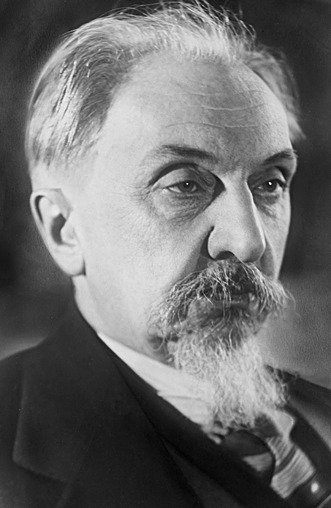
\includegraphics[width=.9\textwidth]{figures/Scerba.jpg}
  \caption{Lev Vladimiovič Ščerba}
  \label{fig:ch.kazan_scerba}
\end{wrapfigure}
The distinctive character of the \isi{phoneme} was further emphasized in its
treatment by his student L. V. {\Ščerba} (1880-1944). {\Ščerba} had studied
phonetics in Paris with Rousselot\ia{Rousselot, Jean-Pierre} and {\Passy} before coming to
St. Petersburg in 1909 to head the laboratory of experimental
phonetics. He subsequently followed {\Baudouin}'s lectures there, though
he was already familiar with his work in general. Since {\Ščerba}'s
interest was most directly in phonetic structure, he was not primarily
concerned with the theory of alternations (though he did write some on
this topic in later years); he did, however, take over from {\Baudouin}
some of the latter's psychological approach to the definition of
phonemes.

Partly on the basis of ideas he may have gotten from {\Passy}'s work,
{\Ščerba} was concerned to emphasize the distinctive or
meaning-differentiating function of phonemes. As a result, he could
not accept {\Baudouin}'s interpretation of these as defined by the full
class of divergences: since [d] and [t] in \ili{German} serve to
differentiate words from one another, it would not do to represent one
and the same sound sequence (e.g. [bunt]) by two different phonemic
forms (/bund/ and /bunt/) depending on morphological relationships. As
a result, {\Ščerba}'s notion of the \isi{phoneme} (which formed the basis of
that associated with the Leningrad school of Soviet linguistics) could
only treat two sounds as belonging to the same \isi{phoneme} if they are
members of a \isi{divergence} which does not neutralize otherwise
distinctive differences.

This is a reasonably natural (though hardly inevitable) development of
{\Baudouin}'s notion, and it was in this form that the linguistic
theories of subsequent years would approach the nature of the
\isi{phoneme}. But, by retaining {\Baudouin}'s psychological perspective on the
\isi{phoneme} as ``a sound of the same intention'' but of ``different
anthropophonic realization'' \citep[171]{baudouin95:attempt}, {\Ščerba}'s
conception acquires another aspect which was not generally
ac\-cepted. It seems quite plausible (indeed, necessary) on this view to
regard the sound which represents the underlying intention of the
speaker as a `basic variant' which is transformed into various
secondary variants under some (but not all) conditions. As remarked
above, the Kazan notion of an \isi{alternation} was not derivational in this
sense (though sometimes {\Baudouin} and {\Kruszewski} do speak,
unsystematically, of one member of an \isi{alternation} as its `basic
variant'). Once we articulate the notion of phonemes as the
psychological invariants underlying (a restricted class of)
divergences, though, it is much more natural to adopt such a
derivational picture, along the lines of the `fully specified basic
variant' view sketched above in chapter~\ref{ch.saussure_sound}.

It was in the form of this `Leningrad school' \isi{phoneme} that {\DeCourtenay}'s views contributed to forming the climate of \ili{Russian}
linguistics in the period around World War I. It is perhaps ironic
that a linguist whose most important and best-developed work in
general linguistics concerned the notion of rule (in the sense of the
present book) should be best remembered for helping to form a
particular notion of \isi{phonological representations}. In any event, the
discussion that centered on the validity of the Leningrad conception
of the \isi{phoneme} was influential in determining the views of a later
generation of linguists, who were in Russia at this time but who would
subsequently form the {nucleus} of the Prague Linguistic Circle.

%%% Local Variables: 
%%% mode: latex
%%% TeX-master: "/Users/sra/Dropbox/Docs/Books/P20C_2/LSP/main.tex"
%%% End: 
